\documentclass[t,10pt]{beamer}
\usetheme[official=true, titlebgimage=RFX-transparent-logo,%
conference=\mbox{N. Vianello
  @ JET 01 June 2012},pagelogo=false]{Rfx}
\usepackage{palatino}
%\usepackage[english]{babel}
\usepackage{listings,amsmath,multimedia}
\usepackage{tangocolors}
\usepackage{rfxcolor}
\usepackage{pgf}
\usepackage{tikz}
%\usepackage[bibstyle=numeric-comp,citestyle=authoryear-comp,labelyear=true,maxnames=1]{biblatex}
%\bibliography{biblio}
%\renewcommand*{\bibfont}{\footnotesize}
\mode<presentation>
\graphicspath{{pdf_box/}}
\renewcommand\Re{\operatorname{Re}}
\renewcommand\Im{\operatorname{Im}}

% for adding foot note with reference
\makeatletter
% add a macro that saves its argument
\newcommand{\footlineextra}[1]{\gdef\insertfootlineextra{#1}}
\newbox\footlineextrabox

% add a beamer template that sets the saved argument in a box.
% The * means that the beamer font and color "footline extra" are automatically added. 
\defbeamertemplate*{footline extra}{default}{
    \begin{beamercolorbox}[ht=2.25ex,dp=1ex,leftskip=\Gm@lmargin]{%
        footline extra}
    \insertfootlineextra
    \end{beamercolorbox}
}

\addtobeamertemplate{footline}{%
    % set the box with the extra footline material
    % \item but make it add no vertical space
    \setbox\footlineextrabox=\vbox{\usebeamertemplate*{footline extra}}
    \vskip -\ht\footlineextrabox
    \vskip -\dp\footlineextrabox
    \box\footlineextrabox%
}
{}

% patch \begin{frame} to reset the footline extra material
\let\beamer@original@frame=\frame
\def\frame{\gdef\insertfootlineextra{}\beamer@original@frame}
\footlineextra{}
\makeatother

\setbeamercolor{footline extra}{fg=structure.fg}% for instance

\title{Research \& Coordination  \\
Activity}
\author{N. Vianello \\
 {\footnotesize Consorzio RFX, Associazione Euratom-ENEA sulla Fusione,
  Padova, Italy}}

\date{ June 01 2012}

\begin{document}

\begin{titleframe}
\end{titleframe}

\begin{frame}{ITER Research Plan framework}
\begin{itemize}
\item European Fusion Research focused on unresolved physical and
technological problems in support of ITER
\item ITER research plan (IRP) individuated 12 top operation risks which 
should be addressed by the world-wide fusion program {\footnotesize
  \textit{(L. Horton FED 2012)}}
\begin{enumerate}
\item \color<2>{verylightgrey} Inadequate disruption mitigation
\item \color<2>{rfxred} H-mode power threshold at high end of
  uncertainty range
\item \color<2>{rfxred} Inadequate ELM mitigation schemes
\item \color<2>{verylightgrey} Inadequate vertical stability control
\item \color<2>{verylightgrey}Lack of reliable high power heating during
  non-active phase of program
\item \color<2>{verylightgrey} Unacceptable divertor performance with tungsten PFCs
\item \color<2>{rfxred} Lack of plasma rotation leading to a
  degradation of plasma performance
\item \color<2>{verylightgrey} High levels of tritium retention requiring more
  frequent tritium removal procedures than foreseen
\item \color<2>{verylightgrey} Incompatibility of core plasma requirements for Q=10 with
  radiative divertor operation
\item \color<2>{rfxred}Inability to achieve densities near
  Greenwald value for required Q=10
\item \color<2>{verylightgrey} Inadeguate particle control to sustain
  high-Q plasma scenario
\end{enumerate}
\end{itemize}

\end{frame}


\begin{frame}{Personal research interest}
\begin{itemize}
{\large\item Actively involved in fusion plasma science since the
M.Sci. thesis in 1999
\item Personal research interests can be summarized into three main
  macro-areas
\begin{description}
\item[(A)] \textcolor{taorange}{Flows \& Turbulence induced transport \\
    $\Rightarrow$ points 2,7}
\item[(B)]\textcolor{ta3chameleon}{Emerging of electromagnetic
    structures  \\
 $\Rightarrow$ points 2,7}
\item[(C)] \textcolor{tascarletred}{3D physics and helical plasmas \\
    $\Rightarrow$ points 2,3,7,10}
\end{description}
}\end{itemize}
\end{frame}

\begin{frame}{Flows \& Turbulence induced transport}


%% per aggiungere la lettera colorata con l'argomento in alto a sx'
\begin{tikzpicture}[remember picture, overlay]
\node [shift={(-0.779 cm,-0.4cm)}]  at (current page.north east)
   {\tikz[baseline=(t1.base)]{\node[fill=taorange](t1){%
{\Large A}};}
    };
\end{tikzpicture}
%%
\begin{itemize}
\item The principal results may be summarized as follows:
\begin{columns}
\onslide<2->{\begin{column}{0.48\textwidth}
{\small \begin{block}{}
(i) Momentum flux generated by off-diagonal terms in the stress
tensor: Reynolds stress, Maxwell stress and non-linear momentum flux
$\langle \tilde{v}_{\perp}\tilde{v}_r\tilde{n}\rangle$
\end{block}}
\begin{center}
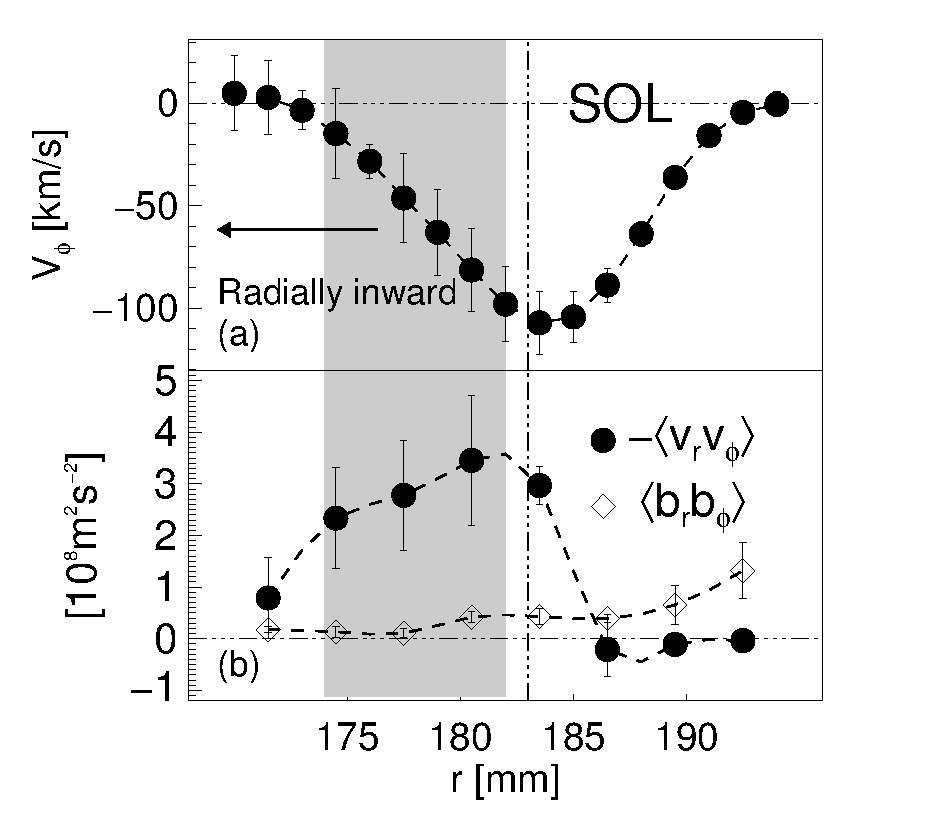
\includegraphics[height=3.4cm]{Profili-Rs-velocity} \\
{\tiny \textit{PRL \textbf{94} (2005), NF \textbf{45} (2005), PPCF \textbf{48} (2006)}}
\end{center}
\end{column}
}
\onslide<3>{\begin{column}{0.48\textwidth}
{\small\begin{block}{}
(ii) Transport reduction induced by active modification of
  sheared flow
\end{block}}

\vspace{.36cm}

\begin{center}
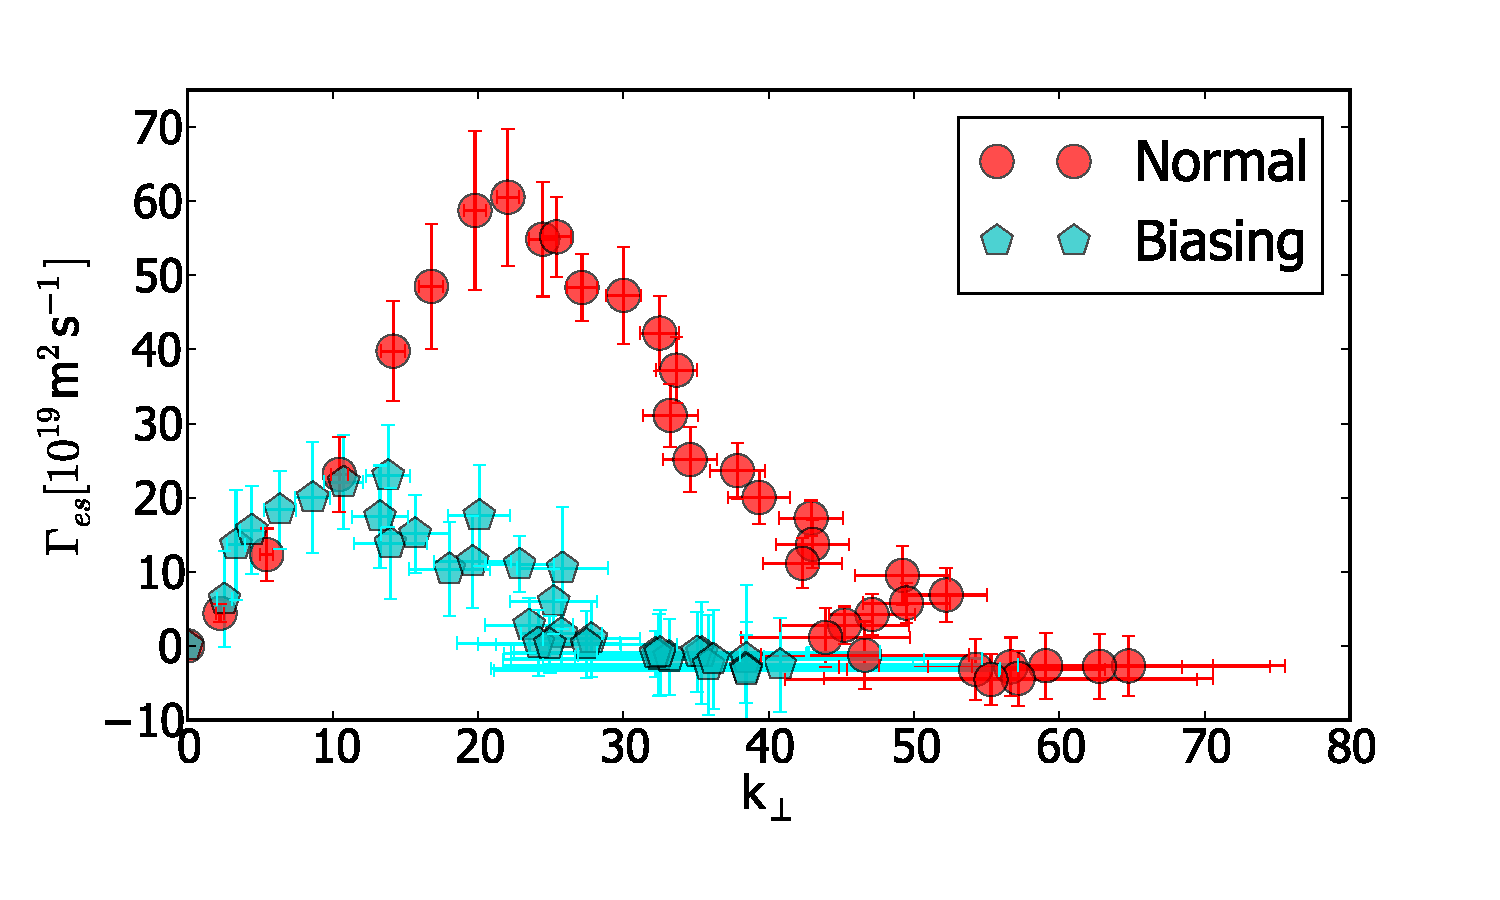
\includegraphics[height=3.4cm]{flux_biasing} \\
{\tiny \textit{PPCF \textbf{42} (2000)}}
\end{center}
\end{column}
}
\end{columns}
\end{itemize}
\end{frame}



\begin{frame}{Coherent structures characterization}
%% per aggiungere la lettera colorata con l'argomento in alto a sx'
\begin{tikzpicture}[remember picture, overlay]
\node [shift={(-0.779 cm,-0.4cm)}]  at (current page.north east)
   {\tikz[baseline=(t1.base)]{\node[fill=ta3chameleon](t1){%
{\Large B}};}
    };
\end{tikzpicture}
%%


\begin{columns}[t]
\begin{column}{0.5\textwidth}
\begin{itemize}
\item Complete electrostatic characterization of intermittent blobs
 
\begin{center}
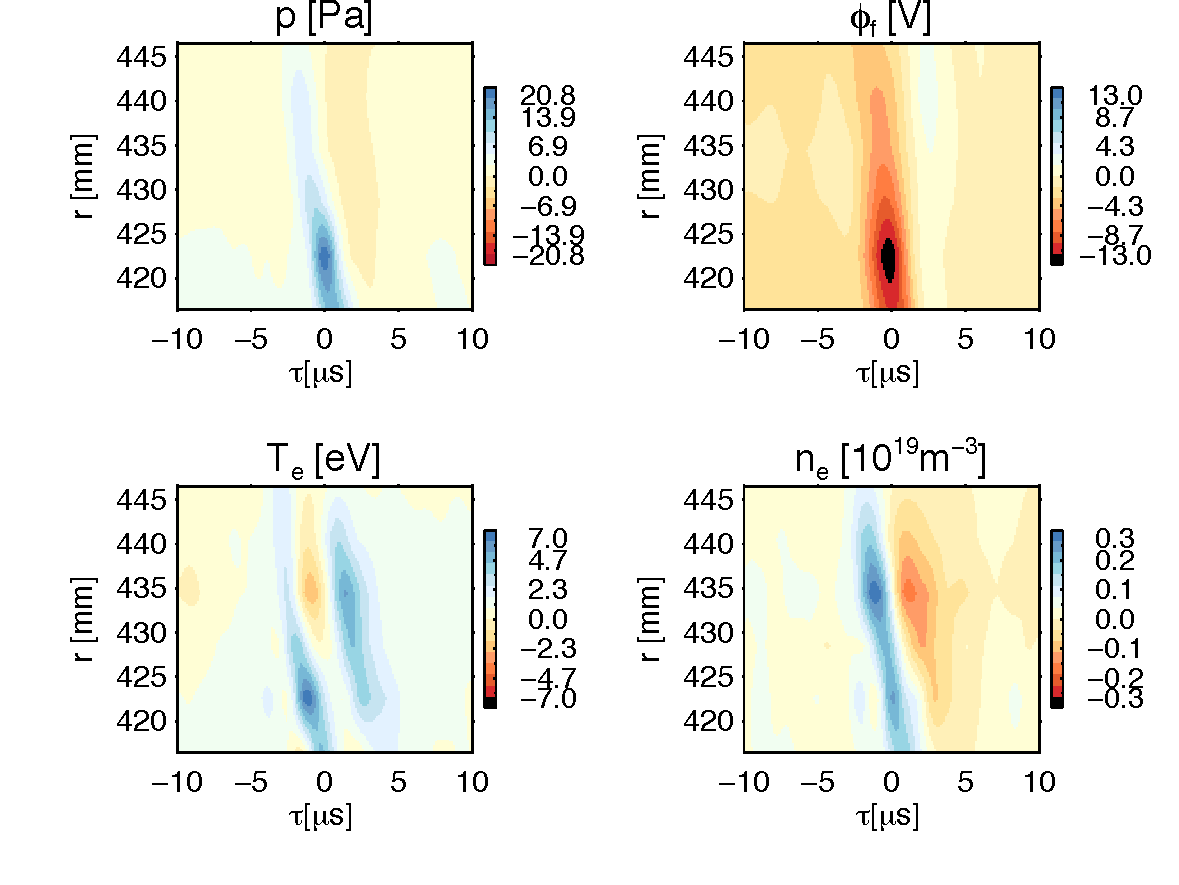
\includegraphics[height=4.5cm]{2Dstructure}\\
{\tiny \textit{NF \textbf{50} (2010)}}
\end{center}
\end{itemize}
\end{column}
\pause
\begin{column}{0.5\textwidth}
\begin{itemize}
\item Evaluation of transport contribution due to coherent structures
\end{itemize}
\begin{center}
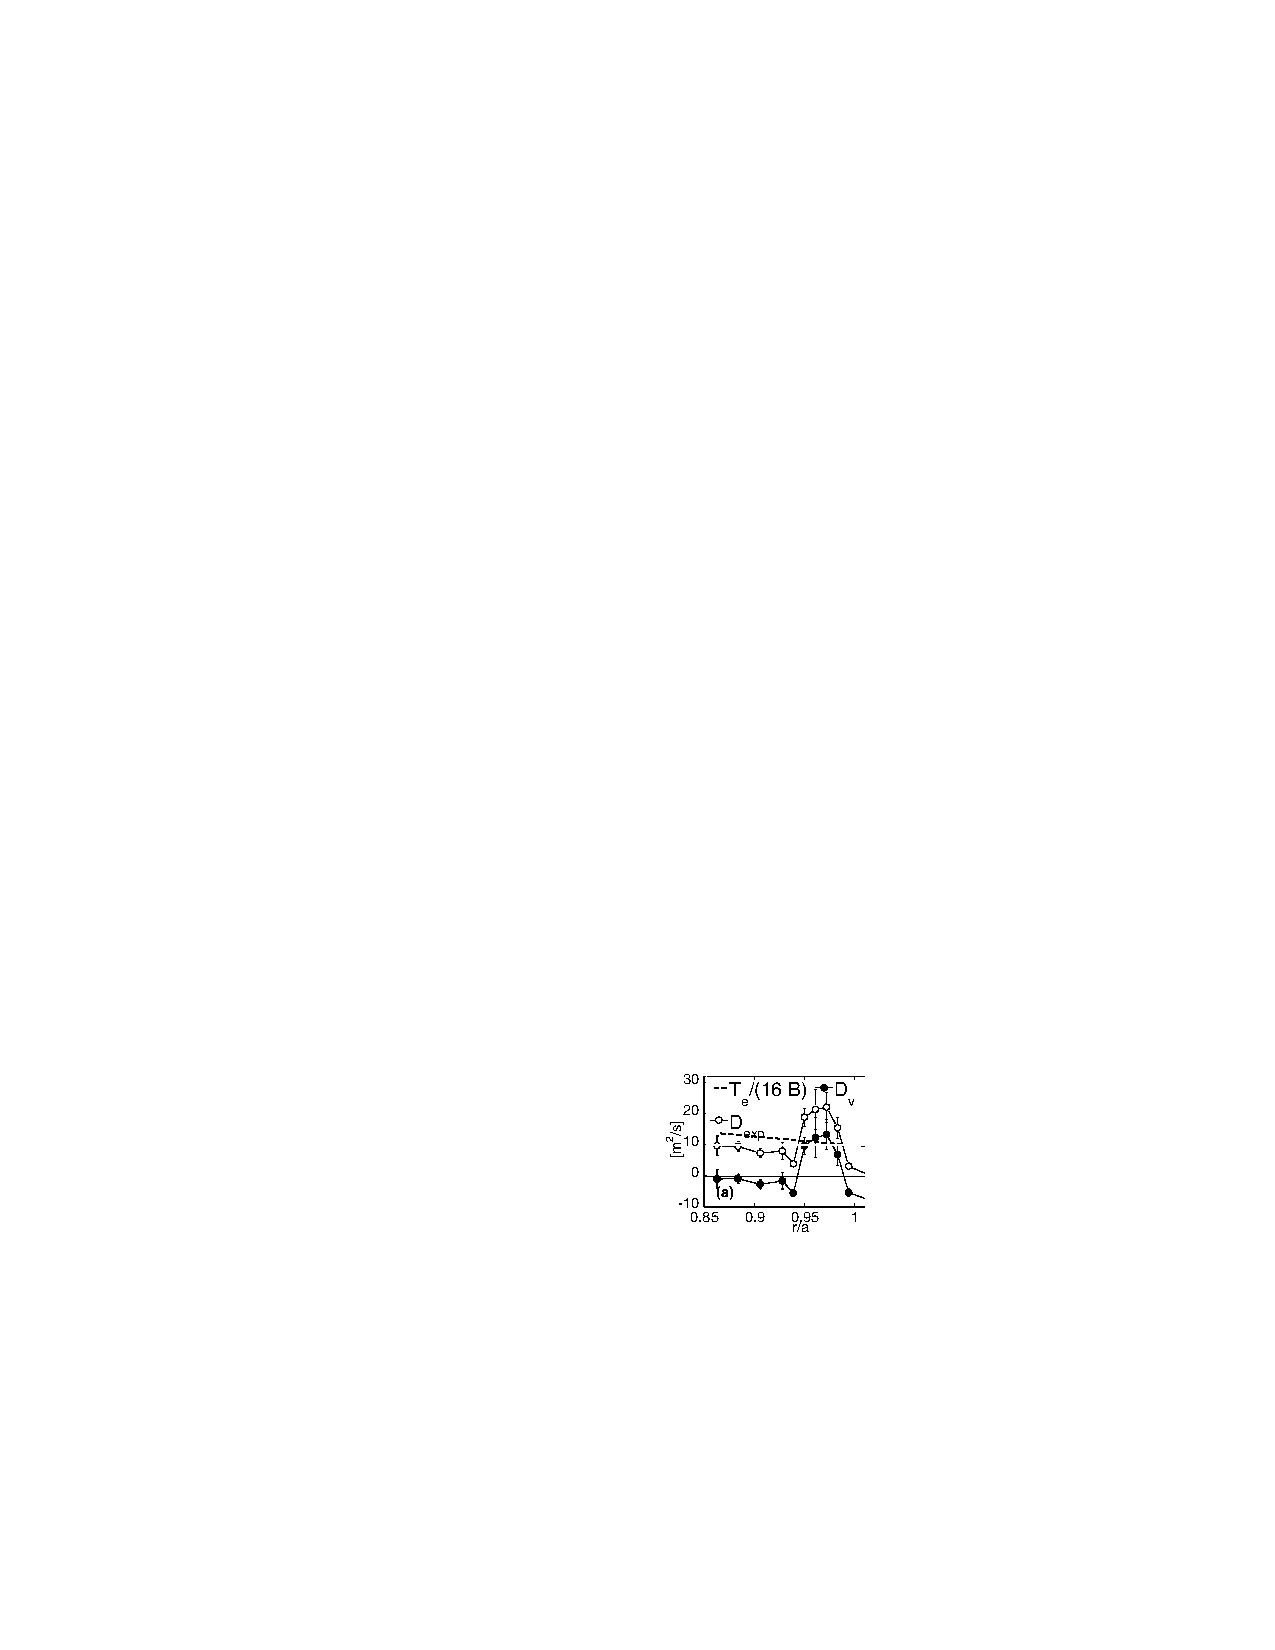
\includegraphics[height=3.2cm]{structure-diffusivity}\\
{\tiny \textit{PRL \textbf{93} (2004), PoP \textbf{9} (2002)}}
\end{center}
\end{column}
\end{columns}
\end{frame}
\begin{frame}{Current filaments}
%% per aggiungere la lettera colorata con l'argomento in alto a sx'
\begin{tikzpicture}[remember picture, overlay]
\node [shift={(-0.779 cm,-0.4cm)}]  at (current page.north east)
   {\tikz[baseline=(t1.base)]{\node[fill=ta3chameleon](t1){%
{\Large B}};}
    };
\end{tikzpicture}
%%
\onslide<1-3>{\begin{itemize}
\item {\small Measurements of parallel plasma current associated to
  \emph{blobs} \& \emph{filaments} in different experiments with
  different magnetic configurations}
\end{itemize}}
\only<1>{
\begin{columns}[c]
\begin{column}{0.6\textwidth}
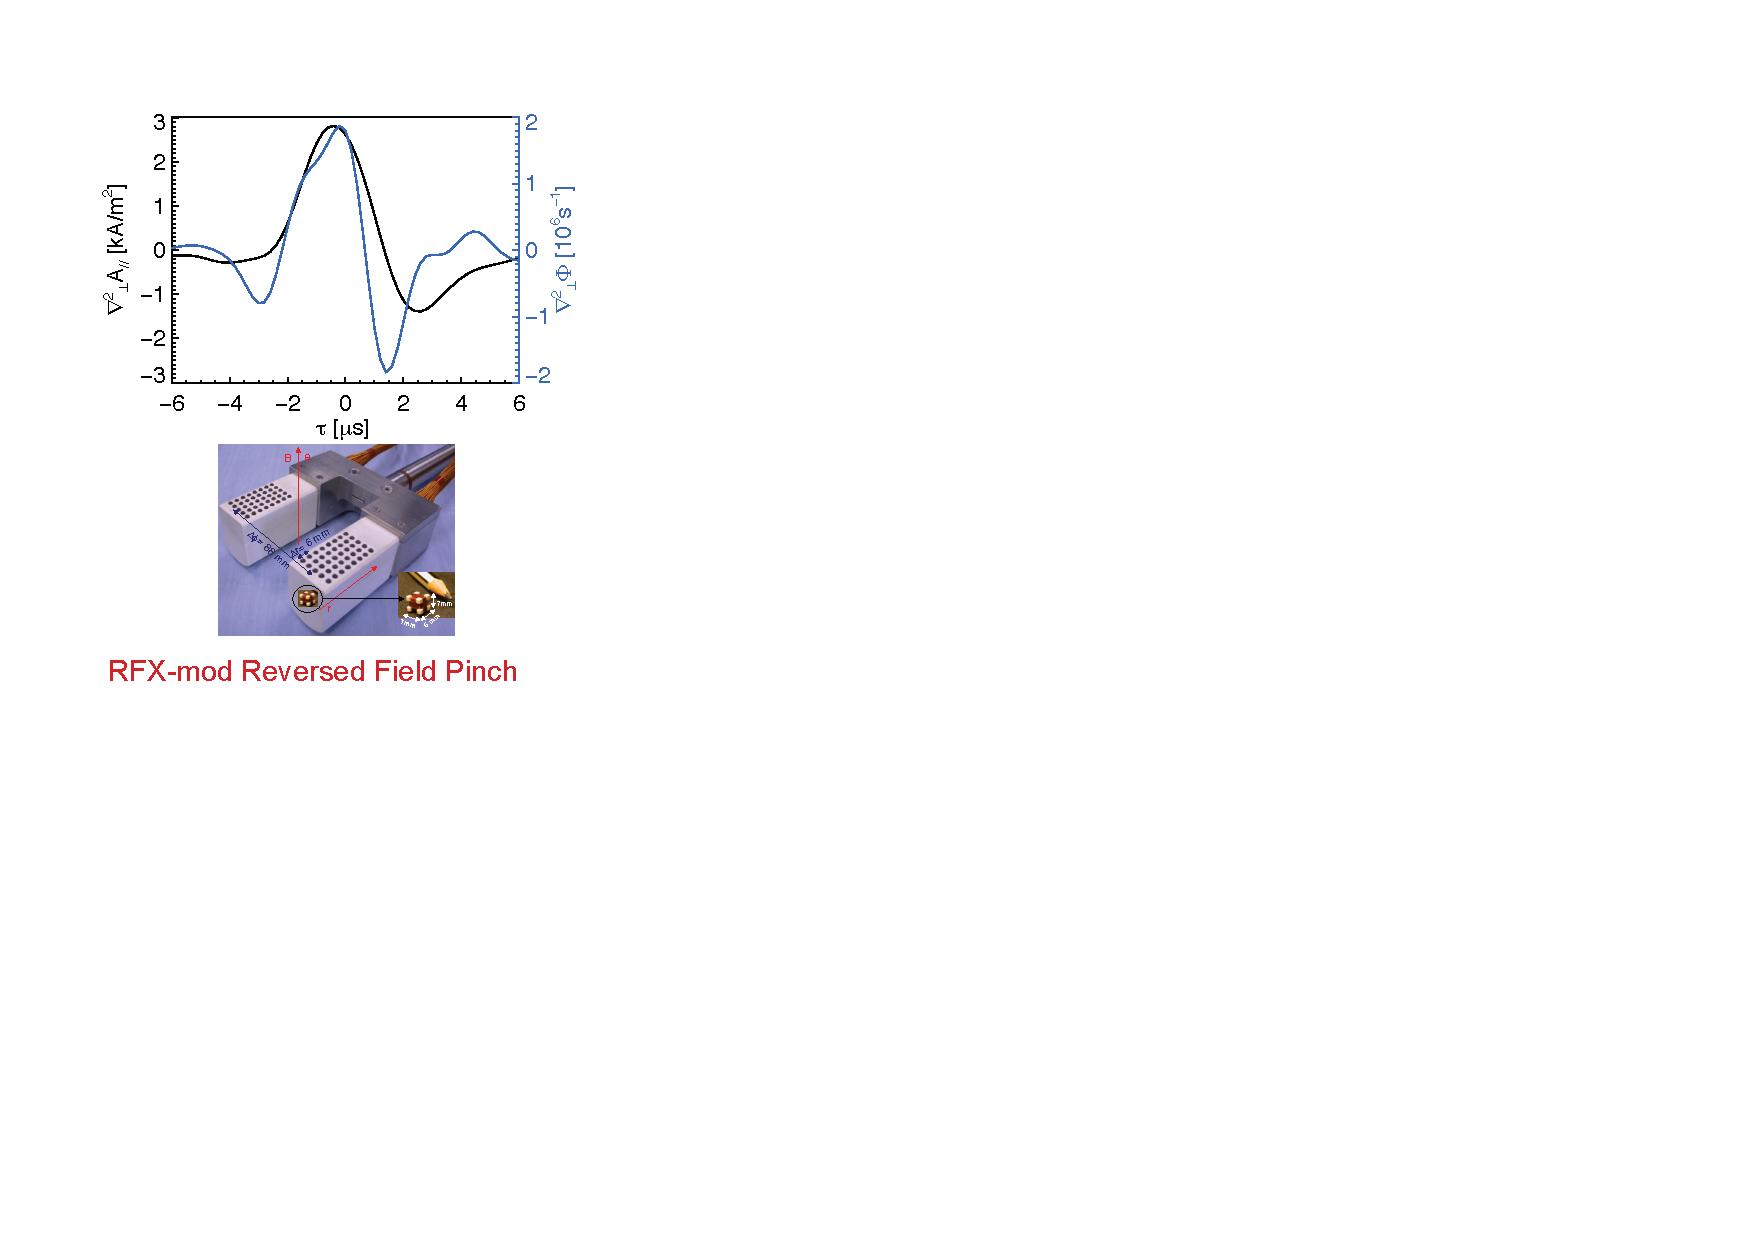
\includegraphics[width=0.81\textwidth]{RFX-current}
\end{column}
\begin{column}{0.4\textwidth}
\begin{block}{RFX-mod Reversed Field Pinch}
\begin{itemize}
\item First direct measurements of current filaments associated to plasma
  blob identified as DKA vortex 
\end{itemize}
{\tiny \textit{PRL \textbf{102} (2009), NF \textbf{50} (2010)}}
\end{block}
\end{column}
\end{columns}
}
\only<2>{
\begin{columns}[c]
\begin{column}{0.6\textwidth}
\includegraphics[width=0.61\textwidth]{AUG-current}
\end{column}
\begin{column}{0.4\textwidth}
\begin{block}{ASDEX-Upgrade Tokamak}
\begin{itemize}
\item First direct measurements of current asociated to type-I
  filaments
\end{itemize}
{\tiny \textit{ PRL \textbf{106} (2011)}}
\end{block}
\end{column}
\end{columns}
}


\only<3>{
\begin{columns}[c]
\begin{column}{0.4\textwidth}
\includegraphics[width=0.78\textwidth]{TORPEX-current}
\end{column}
\begin{column}{0.6\textwidth}
\begin{block}{TORPEX simple magnetized torus}
\begin{itemize}
\item First direct 2D map of parallel current associated to an
  interchange-induced plasma blob 
\end{itemize}
{\tiny \textit{PRL \textbf{106} (2011)}}
\end{block}
\end{column}
\end{columns}

}


\only<4>{\begin{itemize}
\item Collaboration established to extend studies of current filaments
  to other devices, namely \textcolor{ta3chameleon}{\texttt{TJ-II
      stellarator}}, with a probe which combines vorticity and current
  measurements and \textcolor{ta3skyblue}{\texttt{EAST tokamak}} for
  the studies of ELMs
\begin{center}
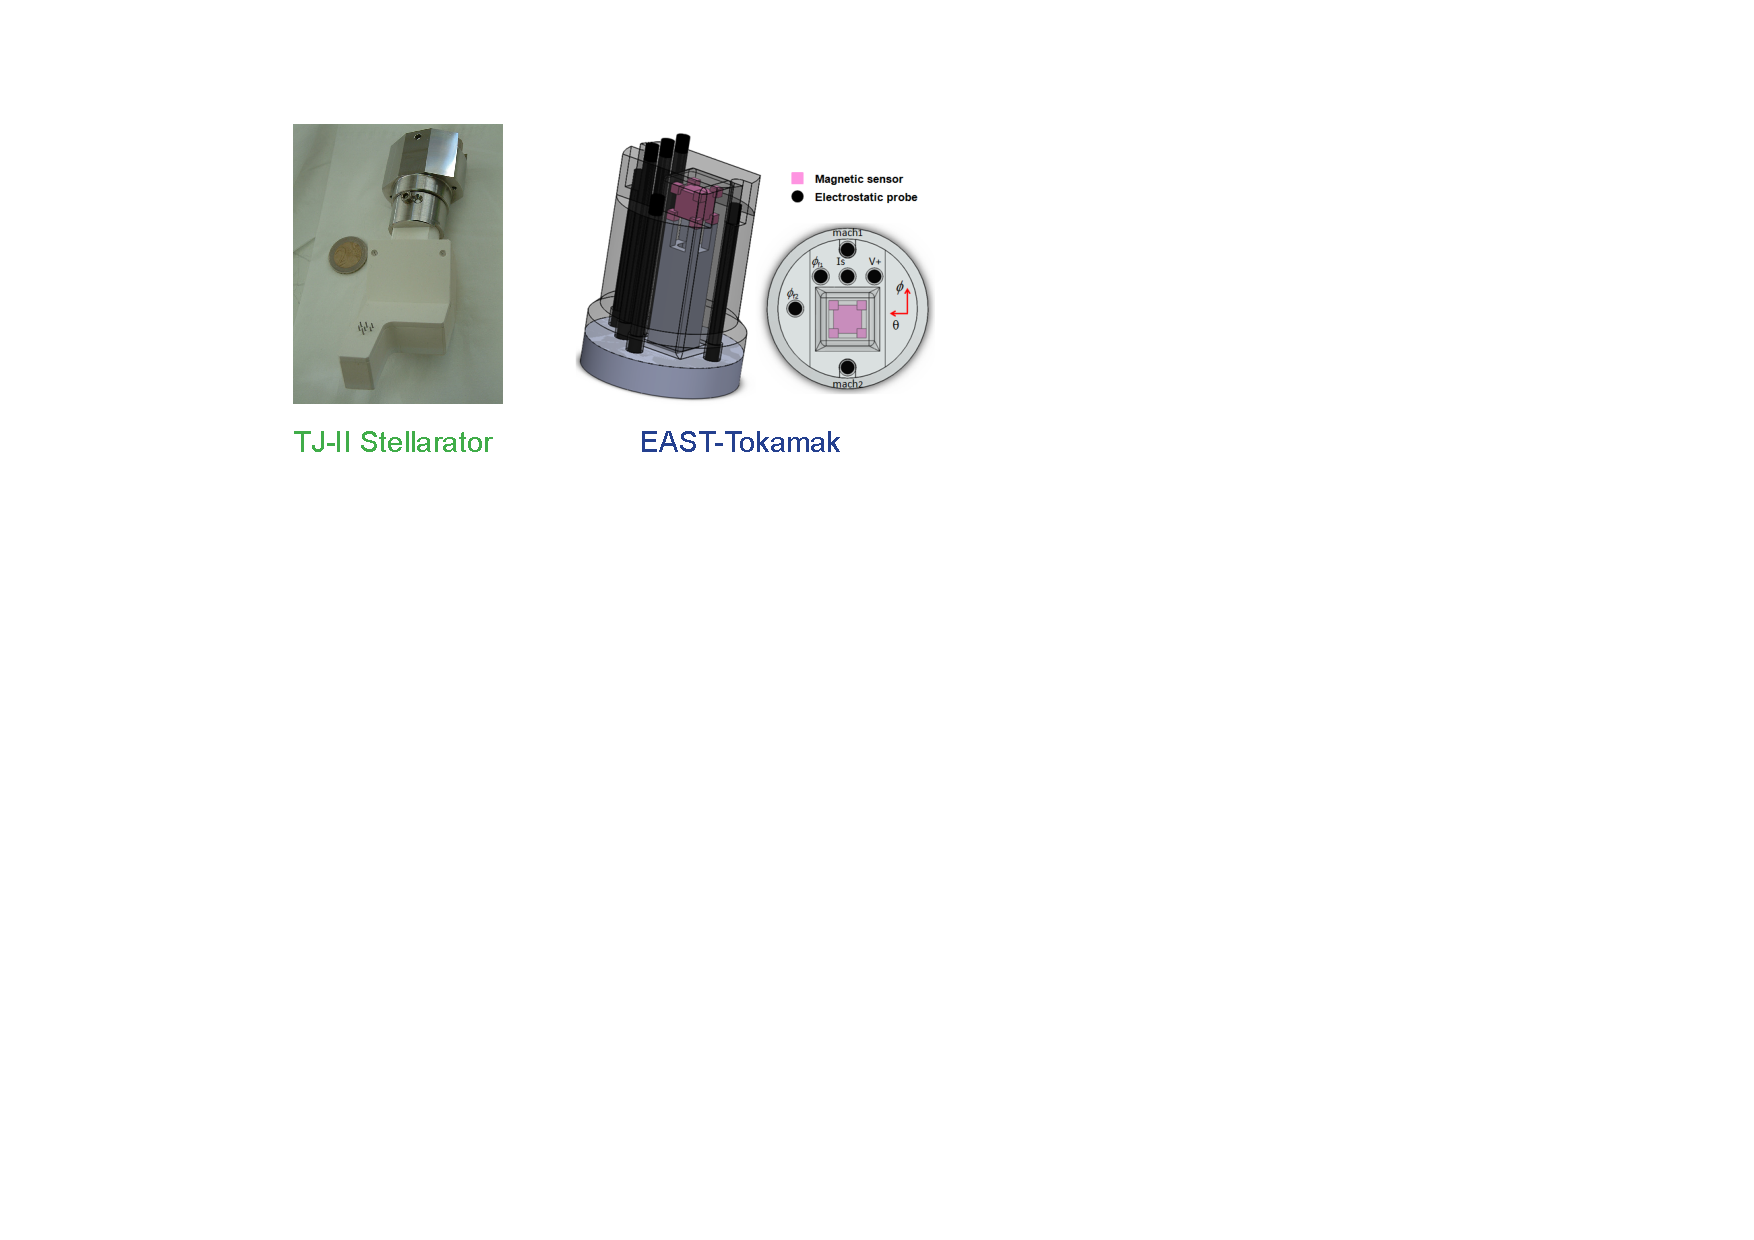
\includegraphics[height=4cm]{collaboration}
\end{center}
\end{itemize}
}\end{frame}


\begin{frame}{Helical plasmas}
%% per aggiungere la lettera colorata con l'argomento in alto a sx'
\begin{tikzpicture}[remember picture, overlay]
\node [shift={(-0.779 cm,-0.4cm)}]  at (current page.north east)
   {\tikz[baseline=(t1.base)]{\node[fill=tascarletred](t1){%
{\Large C}};}
    };
\end{tikzpicture}
%%
\only<1>{
\begin{block}{}
\begin{itemize}
\item {\large Observation and characterization of spontaneous helical plasmas
  developed in high current Reversed Field Pinch operation }
\end{itemize}
{\tiny \textit{Nat. Phys. \textbf{5} (2009)}}
\end{block}
\begin{center}
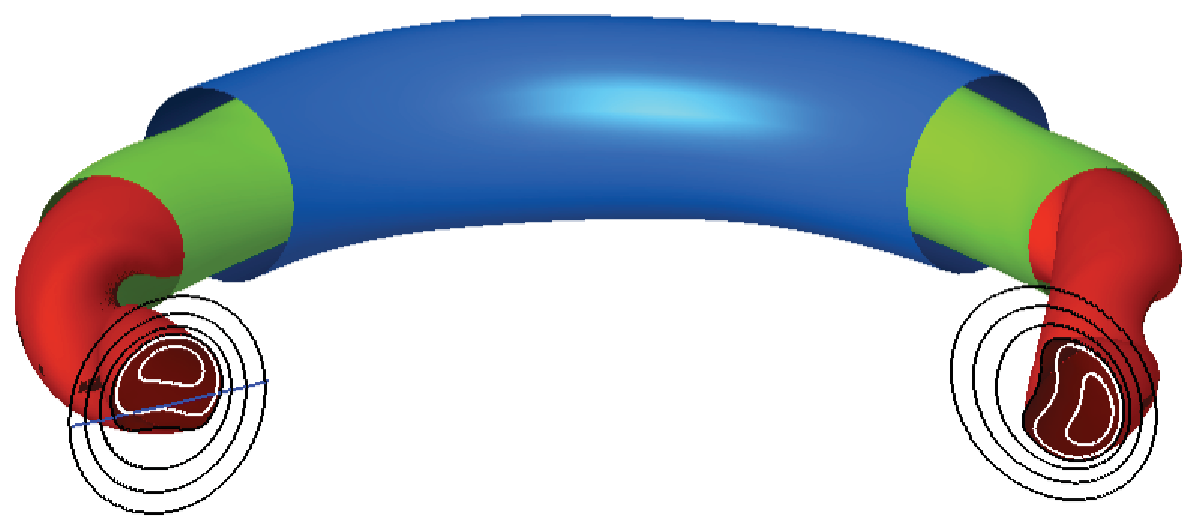
\includegraphics[height=4.3cm]{Torus}
\end{center}
}

\only<2>{
\begin{columns}[c]
\begin{column}{0.5\textwidth}
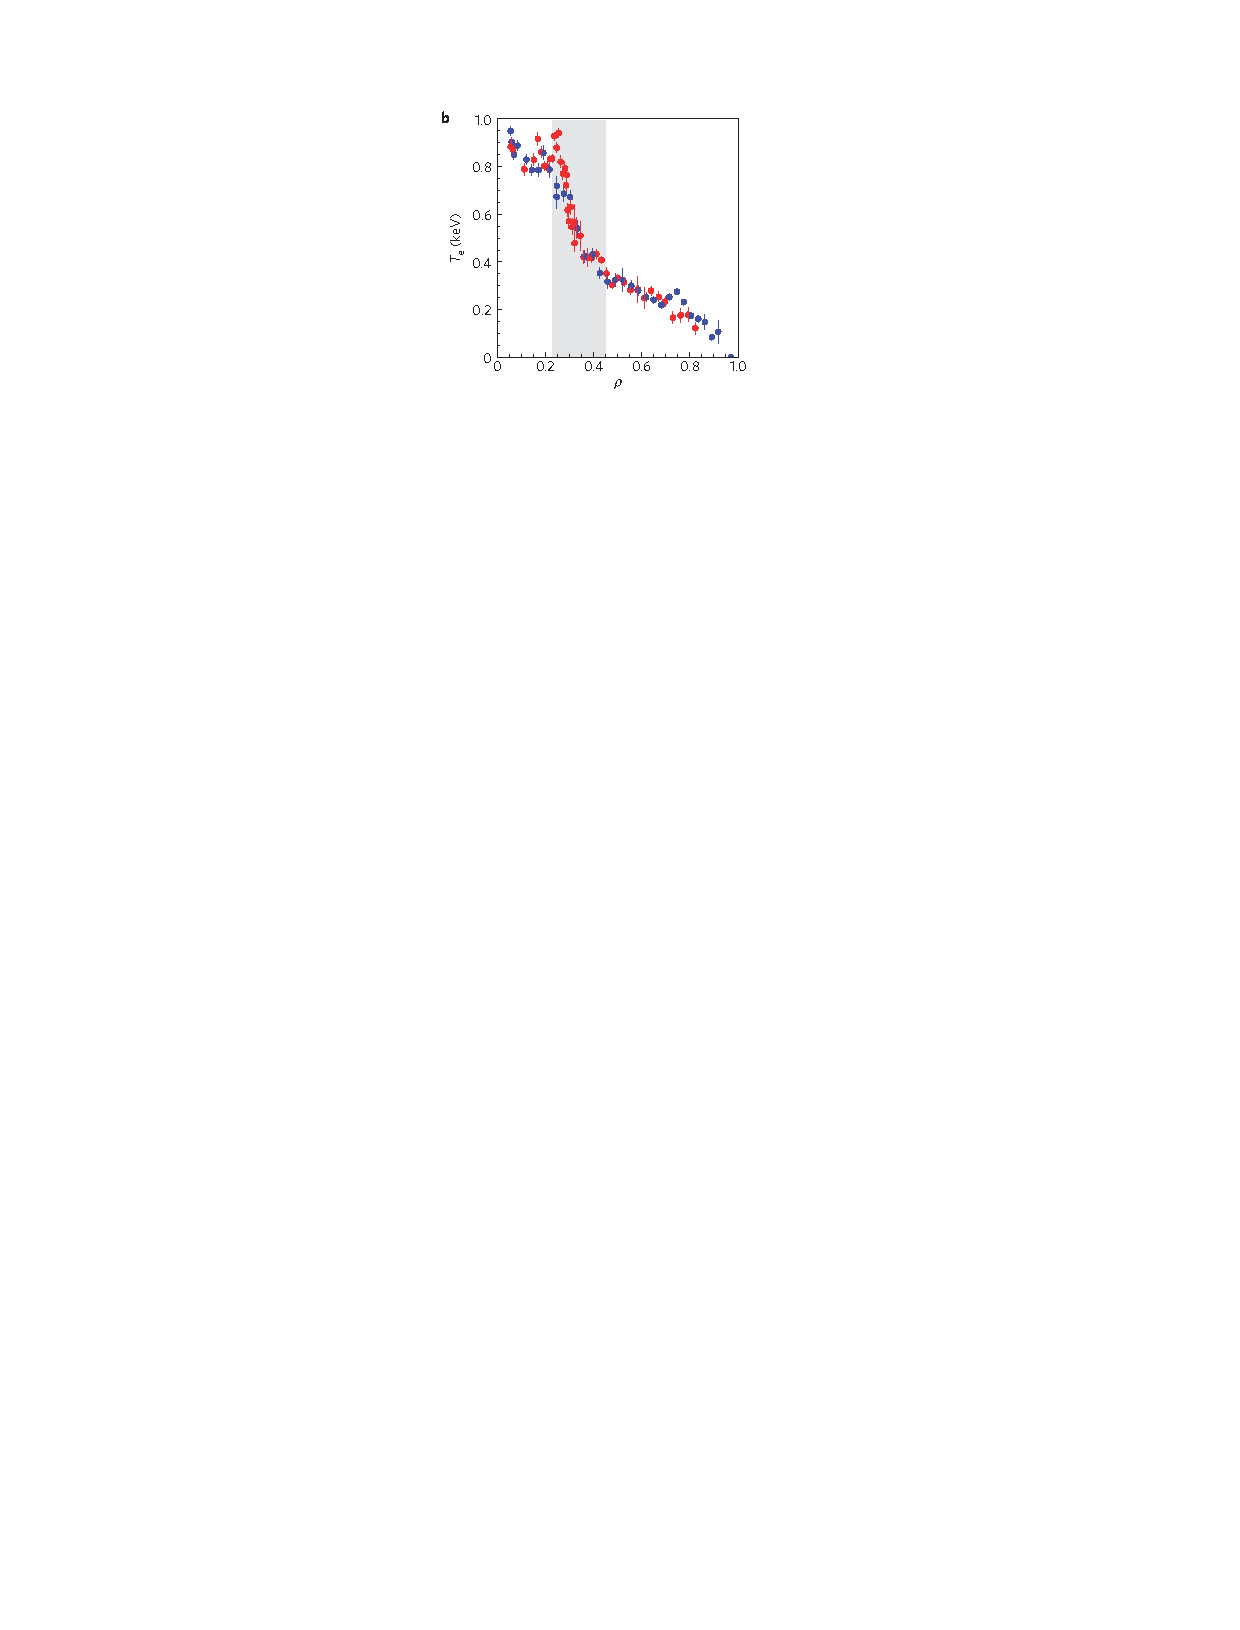
\includegraphics[width=6.cm]{RFX-TraBarr}
\end{column}
\begin{column}{0.5\textwidth}
\begin{block}{}
\begin{itemize}
\item Helical core associated with a transport barrier located in the region
  of a local maxima of $q$ value
\end{itemize}
{\tiny \textit{Nat. Phys. \textbf{5} (2009)}}
\end{block}
\end{column}
\end{columns}
}



\only<3>{
\begin{columns}[c]
\begin{column}{0.5\textwidth}
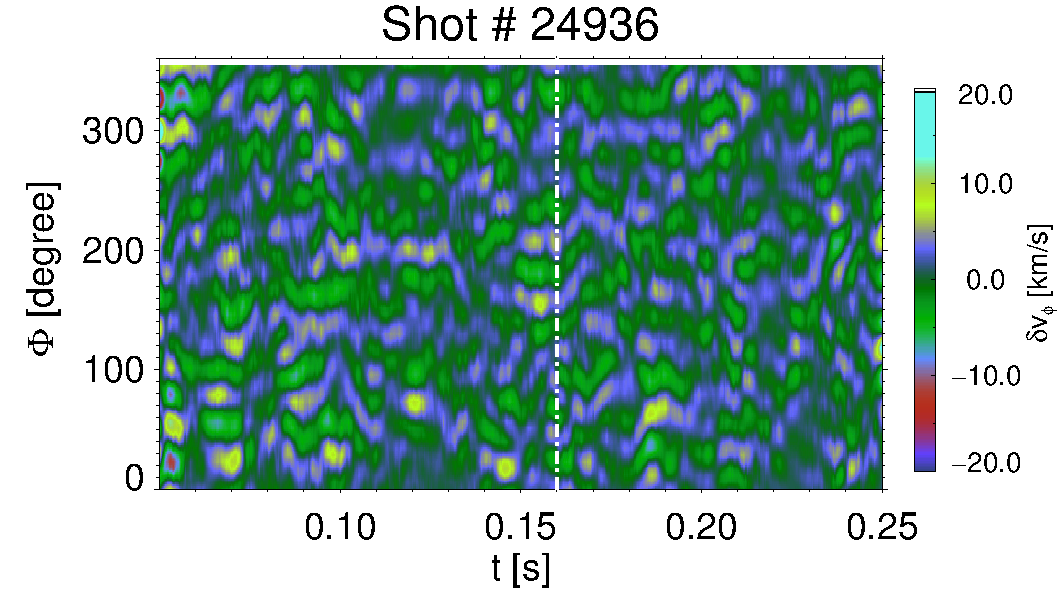
\includegraphics[height=5cm]{helical-flow}
\end{column}
\begin{column}{0.5\textwidth}
\begin{block}{}
\begin{itemize}
\item Ambipolar electric field builds up as a response to the magnetic perturbation
  causing a perpendicular flow with the same periodicity as the
  helical magnetic perturbation
\end{itemize}
\end{block}
\end{column}
\end{columns}
}

\only<4>{
\begin{columns}[c]
\begin{column}{0.5\textwidth}
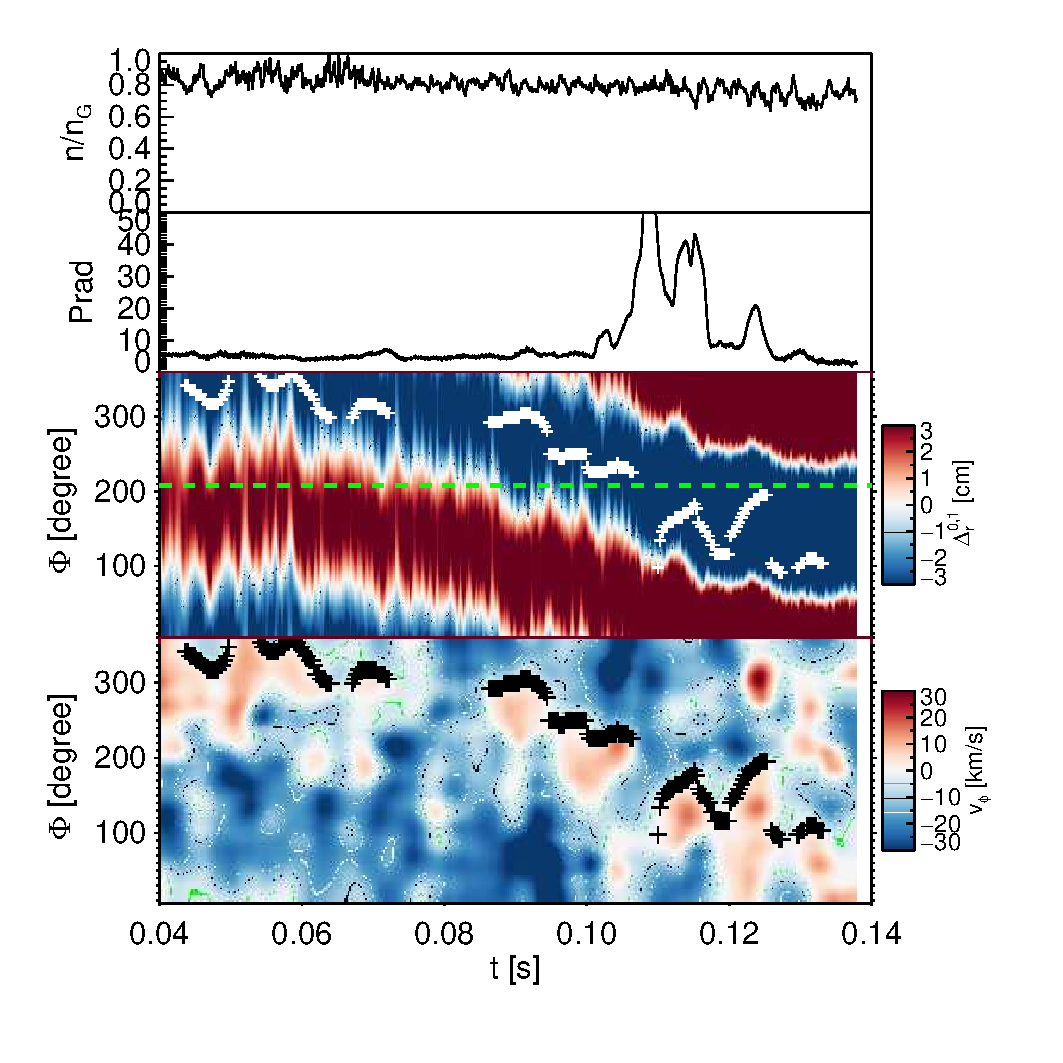
\includegraphics[height=6.6cm]{Shot26317_ShiftFlow}
\end{column}
\begin{column}{0.47\textwidth}
\begin{block}{}
\begin{itemize}
\item Similar phenomenology appears in High density regime
\item In this case, radiative collapse caused by density accumulation induced by perpendicular flow inversion
\item Accumulation point coincides with the X-point of the magnetic
  islands
 \end{itemize}
{\tiny \textit{NF \textbf{52} (2012)}}
\end{block}
\end{column}
\end{columns}
}
\end{frame}


\begin{frame}{JET activities}
\only<1>{
\begin{block}{Toroidal braking during EFCC experiment in ILW}
\begin{itemize}
\item Toroidal rotation braking estiamated from magnetic including
  diamagnetic correction
\item Different braking observed as a function of dosing rate
\end{itemize}
\end{block}
\begin{columns}[t]
\begin{column}{0.5\textwidth}
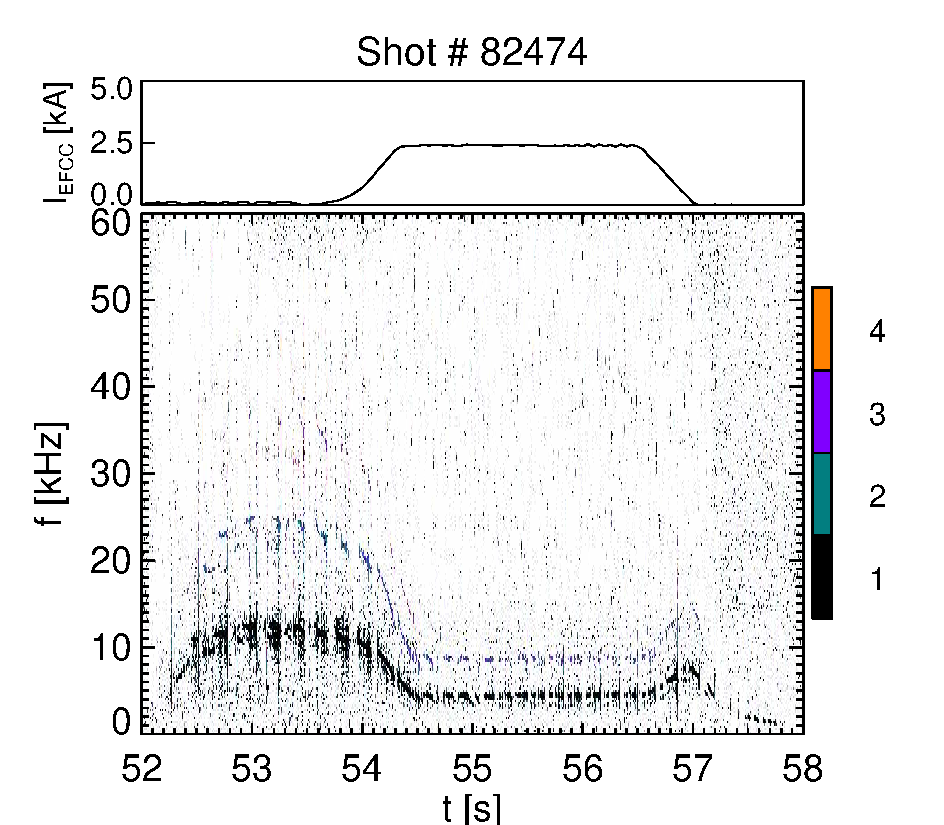
\includegraphics[width=.9\textwidth]{nspectrum82474}
\end{column}
\begin{column}{0.5\textwidth}
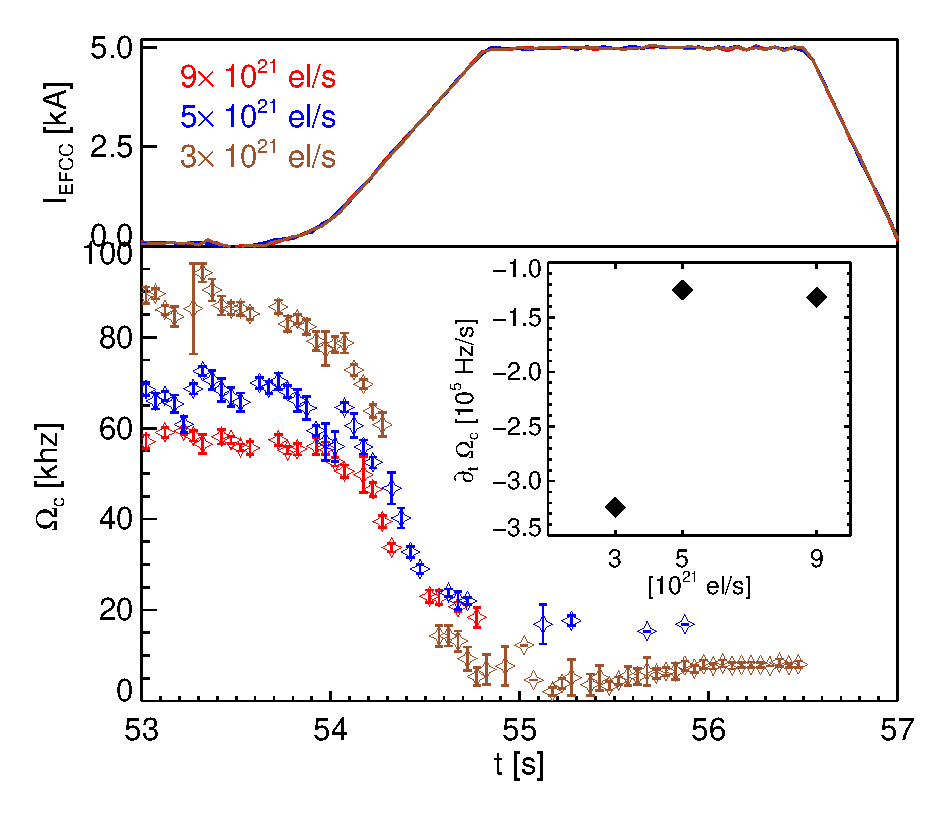
\includegraphics[width=.9\textwidth]{OmegaC_GasPuffScan}
\end{column}
\end{columns}
}

\only<2>{
\begin{block}{Divertor oscillations and M-Mode}
\begin{itemize}
\item ICRH plasmas exhibit oscillations in the divertor D$_{\alpha}$ signals
\item They are sort of \emph{precursor} for the M-mode (m,n)=(0,0)
  mode at few kHz
\end{itemize}
\end{block}

\vspace{1cm}

\begin{columns}[t]
\begin{column}{0.5\textwidth}
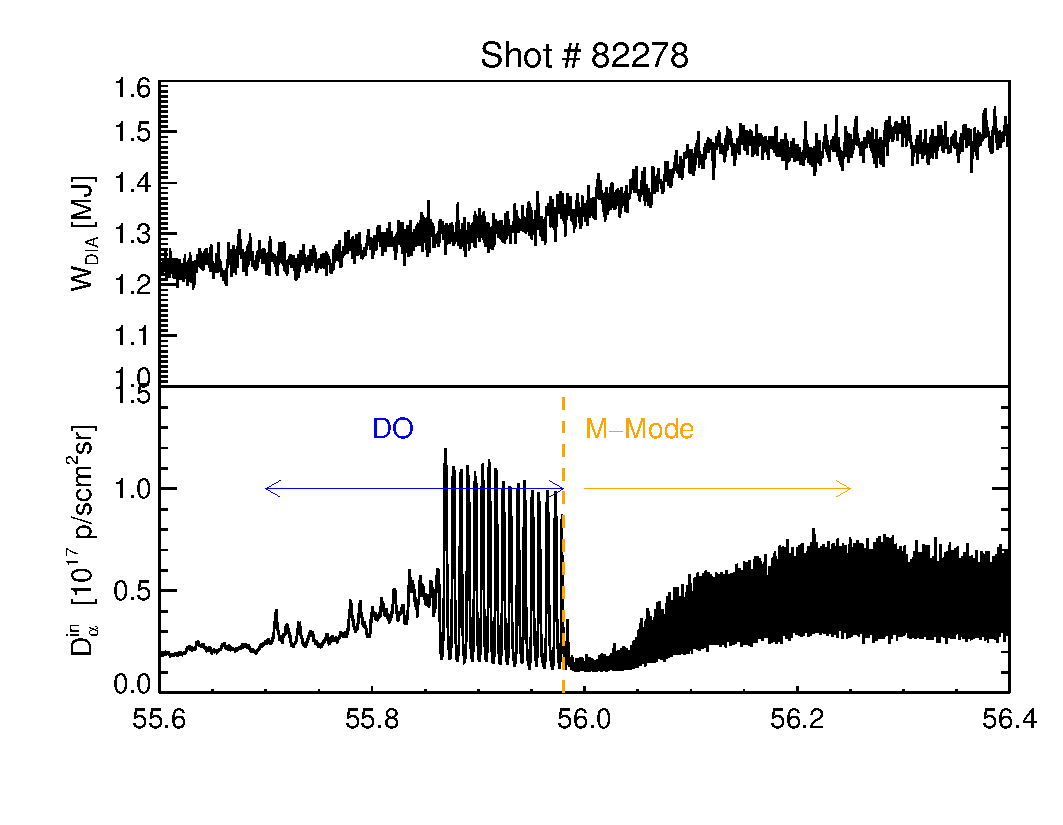
\includegraphics[width=\textwidth]{wdia_dalpha}
\end{column}
\begin{column}{0.5\textwidth}
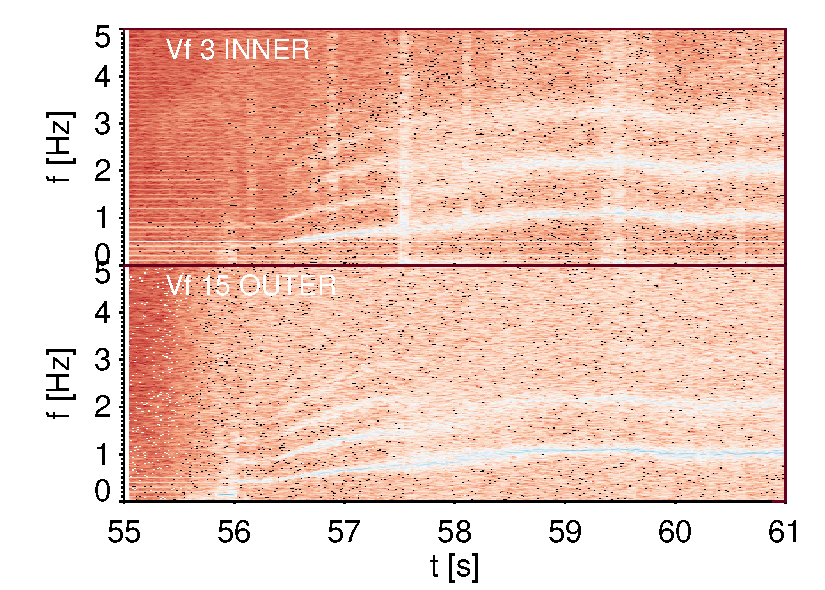
\includegraphics[width=\textwidth]{spectrogramVf}
\end{column}
\end{columns}


}
\end{frame}

\begin{frame}{Coordination experience:RFX-mod}
\begin{itemize}[<+->]
\item RFX-mod scientific program is coordinated by Task Force Leaders in collaborations with
  Scientific Coordinators
\item Scientific objectives are determined on the basis of
  experimental proposals (around 100 experimental proposals for each year)
\item Experimental time allocated on the basis of scientific
  priorities and machine condition in order to optimize the
  experimental time
\item I've been appointed task force leader for two subsequent years:
  \begin{description}
  \item[2009] Task force \alert{Particle, momentum and energy transport}
  \item[2010] Task force \alert{Physics integration for high
      performance RFP}
  \end{description}
\end{itemize} 
\end{frame}


\begin{frame}{Coordination experience: EFDA TTG}
  \begin{itemize}
\item In 2011 I've been appointed as coordinator of the working group
  \emph{3D field effects in edge and SOL and diagnostic development}
  for the EFDA Transport-topical group
\item Duties and responsabilities
  \begin{itemize}
\item Monitoring and coordination of activities from 11 different European Associations
\item Discussion stimulated through remote meetings and shared wiki
  pages information
\item Activities monitored and reported to STAC committee 
  \end{itemize}
\item Programme commitee of the forthcoming 17th Joint EU-US Transport
  Task Force Meeting: chairman of the session on \emph{Edge and SOL
  turbulence and transport}
\end{itemize} 
\end{frame}

\begin{frame}
  \frametitle{Scientific objectives I}
  Using draft of JET 2013 work program the following scientific topics
  have to be pursued
  \begin{description}
  \item[Headline 2.2] \textbf{Assess plasma scenario with regards to
      power loads, their mitigation and control}
    \begin{itemize}
    \item Complete the characterization of the ELMs in ILW. Why do they
      seem \emph{slower}? Is this related to different pedestal
      pressure/current profile?
    \item Determine the plasma flow response to RMPs highlighting
      differences with respect to collisionality. Can eventual differences account for different behavior with respect to
      collisionality?
    \item Determine the role of MHD islands in the density limit. Is
      radiative collapse really determined by density accumulation?
    \end{itemize}
  \end{description}
\end{frame}
\begin{frame}{Scientific objectives II}
\begin{description}
\item[Headline 3.4] \textbf{Confinement pedestal and ELM physics}
    \begin{itemize}
    \item Complete characterization of ILW pedestal.
    \item Determine the
      reason for \emph{cooler} pedestal. Different/enhanced thermal
      transport mechanism?
    \item If the pedestal is the result of a balance between
      $\omega_{E\times B}$ and turbulence determine flow profiles in
      ILW and compare with CW.
    \item Is there any correlation with a different SOL? Different
      neutral profiles determine different conditions at the separatrix?
    \item Why L-H power threshold is lower in ILW? Is it possible to
      relate it to the claimed relation between GAM/turbulence/flow? 
    \end{itemize}
  \item[Headline 3.5] \textbf{MHD and fast particle physics}
    \begin{itemize}
    \item Establish the amount of fast-ion losses caused by RMP
      experiments
    \end{itemize}
  \end{description}
\end{frame}


% \begin{frame}{Scientific topics to be explored}
% \begin{itemize}
% \item Assessment of ITER operation scenarios with the ILW
%   \begin{itemize}
%     \item Complete the characterization of the different physics of ILW with respect to CW
%      \item Why the pedestal is cooler? Is there a different physics?
%     \item Is the SOL different? And what about the separatrix?
%     \item If pedestal is
%     somehow a balance between shear flow and turbulence, what is different? Access to detail investigation
%     of pedestal flow.
%   \end{itemize}
% \item Develop and exploit ELM mitigation techniques:
% \begin{itemize}
%  \item Mandatory is the comprehension of \emph{possible different ELMs}
%  \item Why ELMs are \emph{slower}?
%  \item Establish the dynamics of the recovery phase
%    extending inter-machine comparison also in the recovery phase
%  \item Can the different ELMs be caused by different edge current profiles?
%  \item Role of 3D fields for ELMs for the complete comprehension of RMP mitigation experiments
%  \item Role of 3D fields on the flow: ambipolar response to magnetic perturbation 
%   \end{itemize}
% \end{itemize}
% \end{frame}


\end{document}
